\documentclass[conference]{IEEEtran}
\IEEEoverridecommandlockouts
% The preceding line is only needed to identify funding in the first footnote. If that is unneeded, please comment it out.
\usepackage{cite}
\usepackage{amsmath,amssymb,amsfonts}
\usepackage{algorithmic}
\usepackage{graphicx}
\usepackage{textcomp}
\usepackage{romannum}
\usepackage{enumitem}   


\def\BibTeX{{\rm B\kern-.05em{\sc i\kern-.025em b}\kern-.08em
    T\kern-.1667em\lower.7ex\hbox{E}\kern-.125emX}}
\begin{document}

\title{CS6290: Reading Summary \Romannum{2}}

\author{\IEEEauthorblockN{Yang Ji}
\IEEEauthorblockA{ID:\ 56064832 \\
yangji@comp.hkbu.edu.hk \\
Dept.\ of Computer Science}
}

\maketitle

\section{Summary of Paper \cite{castro1999practical}}


\subsection{Problem Statement}
This paper aims to develop a new replication algorithm to solve Byzantine fault problem efficiently.
%
In particular, it mainly focuses on the asynchronous environment and tries to reduce the response time by adopting many optimizations. 
%
Therefore, how to efficiently improve the system performance without satisfying any security still remained a huge challenge in that era.

\subsection{Problem Significance}
In the distributed system, there is no centralized parties to store and manage node information which can monitor the network running.
%
And some network nodes might perform a wide variety of Byzantine behaviors like message delay, corruption, crashes and so on.
%
Hence, it is of significance for a peer-to-peer network to reach a final consensus in an efficient manner.
 
\subsection{Preliminaries}
\subsubsection{Replication} 
Replication can be used to improve the performance and fault tolerance in the distributed system.
%
It has two basic modes: passive and active.
%
(\romannum{1}) Passive replication (also called primary-backup or master-slave replication) adopts an operating mode in which the primary server is responsible for receiving requests from clients and transmits these requests to the back-ups. 
%
(\romannum{2}) Active replication (also called state machine replication, SMR) ensures that all synchronized servers execute the same set of operations in the same order.

In the traditional Byzantine fault tolerance problem, SMR is applied to ensure the correctness of the whole system due to the failure check of message integrity.
%
Afterwards, introduced public-key cryptography makes BFT with passive replication real.

\subsubsection{Message Authentication Code (MAC)}
In cryptography, message authentication code (MAC) is used to ensure the massage's data integrity and authenticity.
%
In particular, it consists of three main algorithms:

\begin{enumerate}[label=(\roman*)]
    \item \textbf{Key-Generator.} Given a security parameter $1^{\lambda}$, it outputs a key $k$.
    \item \textbf{Signing.} Using the key $k$, it can output a tag $x$ according to the message $m$.
    \item \textbf{Verifying.} Given a tuple $(k, m, Signing(k, m))$, it outputs a decision bit (0 or 1) to tell whether the message m is authentic.
\end{enumerate}

\subsection{State of the Art}
At that time, some protocols implemented in the system SecureRing and Rampart were mainly based on the strong assumption of the synchrony network.
%
The safety could be compromised when there exists malicious attacks from some corrupted nodes.
%
What's more, the cryptographic overhead of public-key scheme could be seen as the major latency in Rampart. 

\begin{figure}[ht]
    \centering
    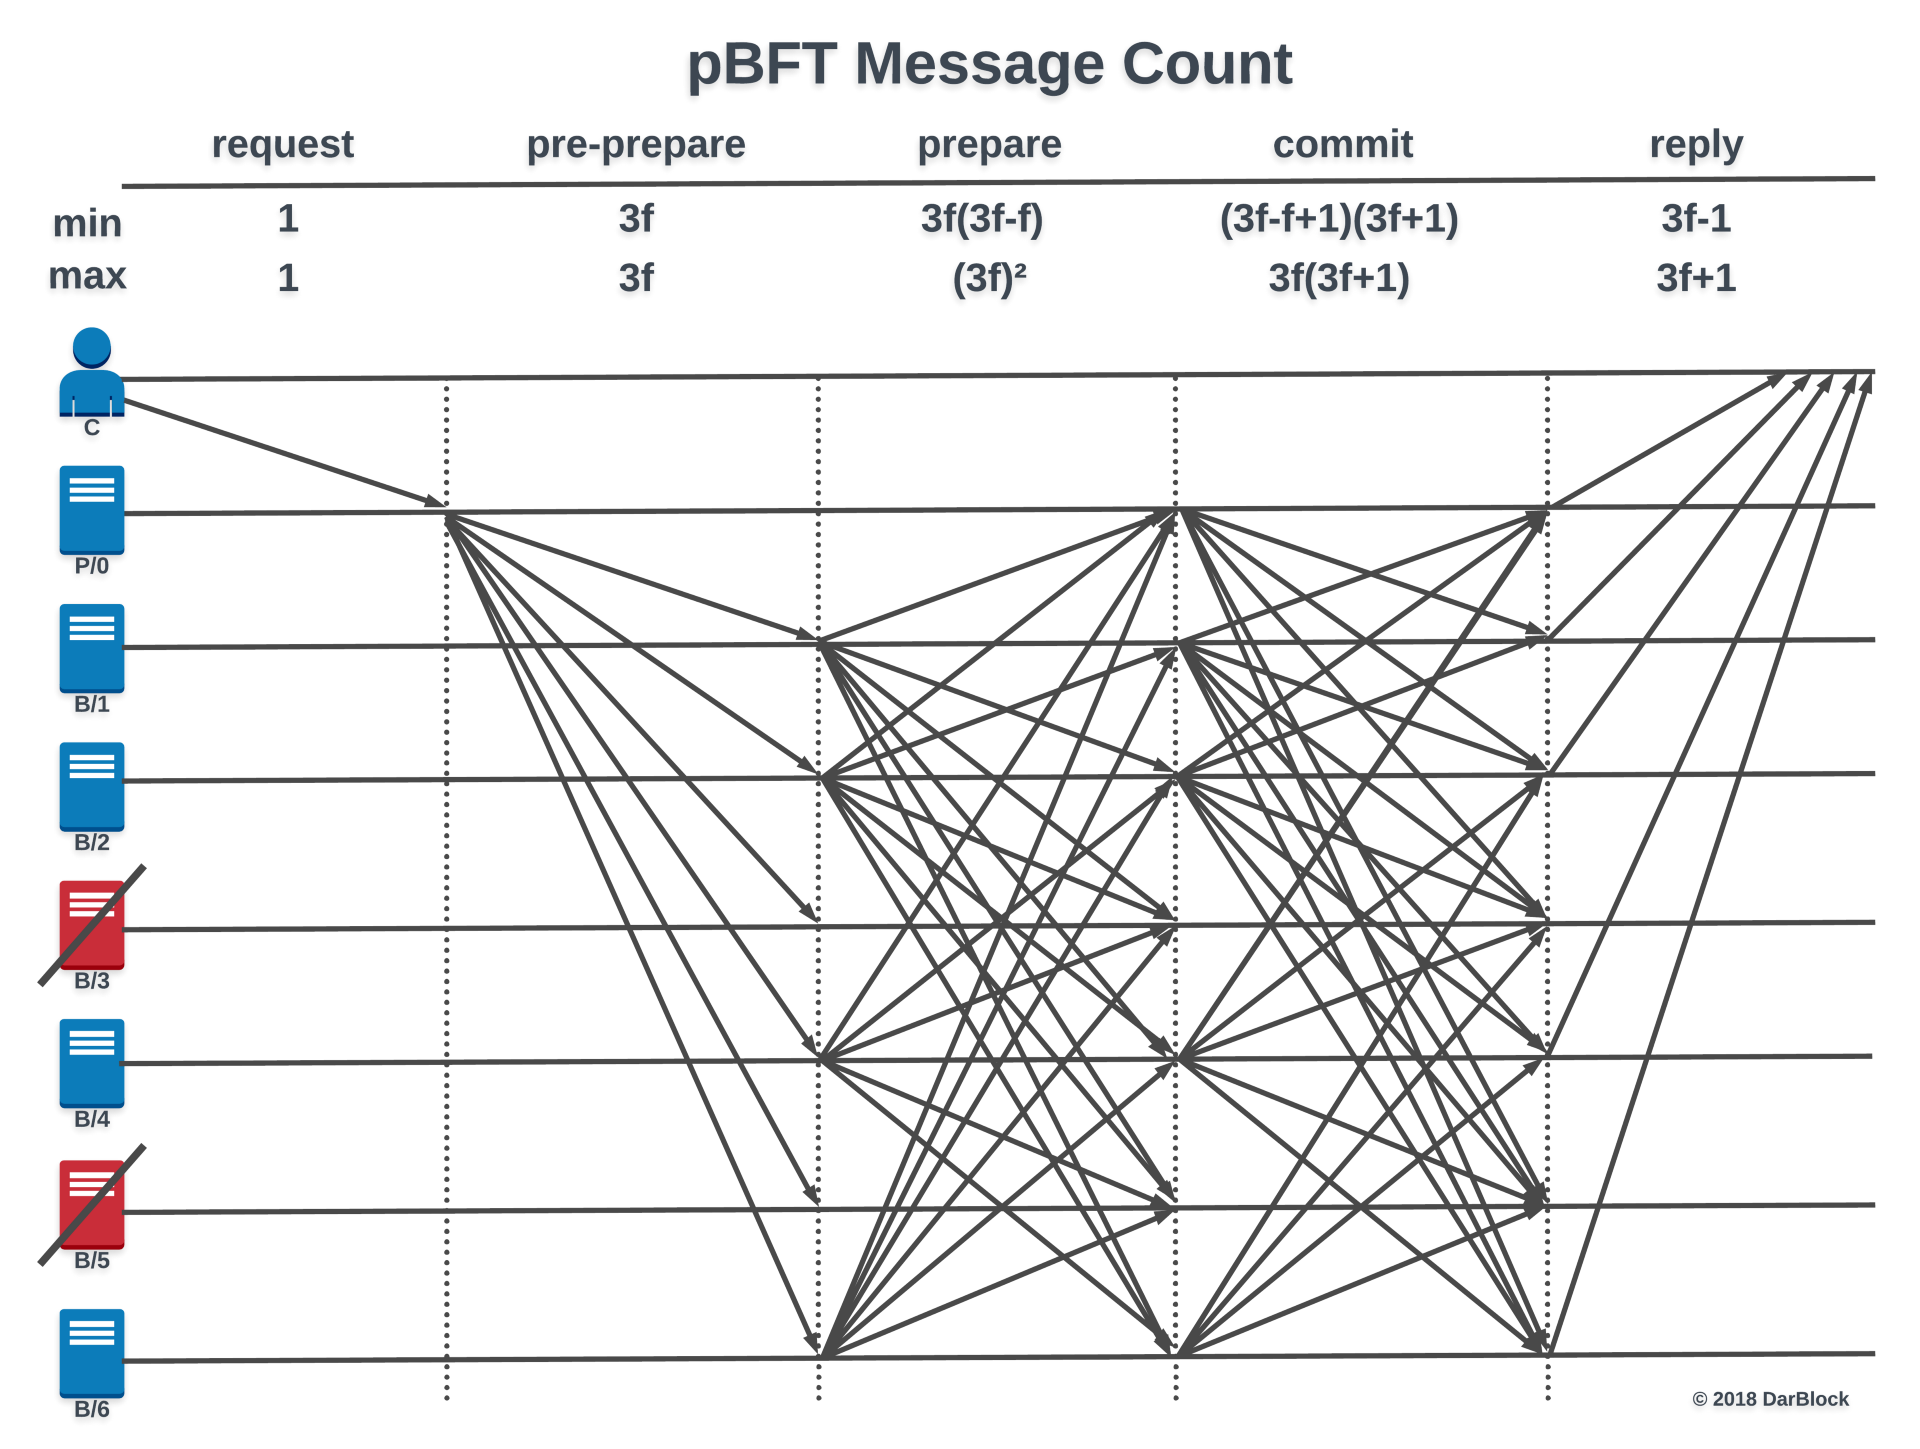
\includegraphics[width= 0.95\linewidth]{fig/PBFT.png}
    \caption{Normal Case Operations}
    \label{pbft}
\end{figure}

\subsection{Contributions}
The goals of three phase protocols are two-fold.
%
One is to establish the total order of execution of requests in the pre-prepare and prepare phase.
%
The other one is to ensure that requests are ordered consistently across views (configurations of replicas with a primary $p = v\ mod\ {\mid} R \mid$ by the commit operations.

The algorithm adopted in this paper is actually a variant of state machine replication shown in Figure\ref{pbft}, including request, pre-prepare, prepare, commit and reply.
%
And it can be concluded as follows:

\begin{enumerate}[label=(\roman*)]
    \item \textbf{Request.} In this period, the client sends a request to the primary server.
    \item \textbf{Pre-prepare.} Upon receiving a new request, the primary node will assign the request a sequence number and then broadcasts this to all replicas. 
    Backup nodes won't accept this request unless the view number, sequence number and tag (message integrity) is valid.
    \item \textbf{Prepare.} After backup nodes accept ${<}pre{-}prepare{>}$ message, it multicasts a ${<}Prepare{>}$ message acknowledgement.
    And this predicate will be accepted only if a replica collects $2f+1$ valid and distinct message. This phase is aimed to ensure the consensus on the sequence number among replicas. 
    In other words, it guarantees that any different messages never have the same sequence number.
    \item \textbf{Commit.} The commit phase is introduced to ensure the total order (consistency) across the views. 
    When receiving $2f+1$ valid and distinct ${<}commit{>}$ messages, the replica could claim that the whole network has reached the consensus.  
    If the primary is suspected as a malicious node, backup servers may request a view change. 
    \item \textbf{Reply.} After the right execution of client's request, the backup node would reply to the client with corresponding answers.
\end{enumerate}

The above five algorithms jointly provide the safety and liveness of the whole system.
%
The safety means that all honest replicas reach the consensus finally, otherwise they will detect the primary is faulty.
%
And the liveness means that the whole system cannot be blocked by the faulty nodes forever (Replicas would move to a new view).

\subsection{Remaining Questions}
The main problem of this three-phase protocol is its communication overhead. 
%
Since its algorithm complexity is $O(n^2)$, the system based on BFT and state machine replication has poor scalability.
%
Unlike the high scalability of Proof-of-Work consensus, it only supports very limited nodes in the network.


\section{Summary of Paper\cite{croman2016scaling}}

\subsection{Problem Statement}
This paper tries to explain and analyze the possible solutions on efficiently scaling current blockchain systems, including parameter tuning and reconstruction of a scalable blockchain.

\subsection{Problem Significance}
As a cryptocurrency system, current blockchain needs to improve the capacity of dealing with transactions.
%
Take Bitcoin as an example.
%
In Bitcoin network, miners need 10 minutes or more to publish a new block and confirm 7 transactions per second at most.
%
In comparison, visa credit card which is a mainstream payment processor can deal with about 2000 transactions per second.
%
The huge gap between blockchain system and traditional payment processor incentivizes blockchain developers to rethink how to scale up network efficiently.

\subsection{State of the Art}
This article reviews the current technologies on scaling blockchains from two perspectives.
%
For one thing, reparameterization of block size and intervals can be viewed as a temporary and limited approach to more scalable blockchains.
%
For another thing, a radical reconstruction of blockchain systems might be the fundamental solutions on scaling up the throughput of blockchains.  
%
Before concluding the analysis of these approaches, I firstly will introduce some preliminaries on network measurement.

\subsection{Preliminaries}

\subsubsection{Maximum Throughput} It describes the maximum quantity of transactions which blockchains could confirm. In general, it is mainly adjusted by the block size and inter-block intervals.

\subsubsection{Latency} Based on the pre-defined consensus protocol, a new block containing variety of transactions needs to wait for around 10 minutes to be confirmed determinately.

\subsubsection{Bootstrap Time} It records the time that a newly joint node needs to prepare for validating the current network status. For Bitcoin, this time is roughly 4 days.

\subsubsection{Cost per Confirmed Transaction (CPCT)} CPCT represents the average cost of confirming a new transaction in the form of USD. 
%
In more details, the cost could derive from the following four sources: (i) Mining (ii) Transaction validation (iii) Bandwidth (iv) Storage.

\subsubsection{X$\%$ Effective Throughput} Here, authors define this concept as (block size) / (X$\%$ block propagation delay) which means that (100-X)$\%$ of the nodes in the network are unable to receive blocks correctly.


\subsection{Contributions}

\subsubsection{Parameter Tuning} 
To be more precise, we could adjust the block size (decides to contain how many transactions in each block) and inter-block intervals actually. 
%
However, we can't increase the block size and reduce intervals infinitely.
%
In order to keep the property of decentralization in the whole system, X$\%$ effective throughput should be at a relatively high level.
%
In other words, if X is fixed on 90, what we could do is just to increase the block size or reduce the inter-block intervals unilaterally.
%
And there exists two main limits on current overlay network:

\begin{itemize}
    \item \textbf{Throughput Limit.} Assume that the inter-block interval is 10 minutes, the block size should not exceed 4MB which can support up to 27 transactions per sec.
    \item \textbf{Latency Limit.} In order to thoroughly employ the bandwidth of the network, the block intervals should be smaller than 12 second.
\end{itemize}

\subsubsection{Hierarchical Design of a Scalable Blockchain}
The paper concludes this design from five perspectives: Network, Consensus, Storage, View and Side planes.

\begin{itemize}
    \item \textbf{Network Plane.} The main reason for latency in Bitcoin is the duplex transmissions at the node level. 
    Nodes need to validate local transactions before publishing this new block.
    A set reconciliation protocol and a centralized, high-speed relay network specially for miners' communication can be possible approaches to this problem.
    \item \textbf{Consensus Plane.} This network plane is aimed to achieve the consensus in the whole network. 
    Many alternatives can substitute PoW protocol to improve the network performance, like GHOST, PoS et al.
    It is worth nothing that sharding (splitting up the problem of consensus) or delegation of trusted and hierarchical sidechains might be a potential solution.
    \item \textbf{Storage Plane.} It provides the storage service for the consensus plane. Operations might include writing, deleting and reading.
    \item \textbf{View Plane.} Authors put forward two potential approaches including nodes replication and data outsourcing.
    \item \textbf{Side Plane.} Side plane provides a off-chain method to realize the payment in a more efficient manner. 
    Through pre-established channels, it solves the inherent problems by introducing a centralized approach.
\end{itemize}

\subsection{Remaining Questions}
Although with these potential solutions on scaling up the blockchain system, it still remains a huge challenge of coordinate the whole system in an efficient manner.
%
What's more, how to persuade the majority to accept a hard fork is another difficult task for the community. 

\bibliographystyle{IEEEtran}
\bibliography{references}


\end{document}
